%%%%%%%%%%%%%%%%%%%%%%%%%%%%%%%%%%%%%%%%%%%%%%%%%%%%%%%%%%%%%%%%%%%%%%%%%%%%%%%%
\section{Methodology/Design}
\label{sec:methodology}

\subsection{Error Injection}
In order to simulate bit flips, we load the model parameters, inject errors into them, save the injected weights,
and load the new weights into a perturbed model. 

To achieve this, we use PyTEI, which provides a flexible API that can generate bit error maps for each part of the model parameters. 
First, we generate bit masks for all parameters we wish to inject into, with one boolean value for each bit in the parameter when stored as IEEE floats.
Then, we specify the probability of a simulated SDC error occuring in the affected parameters, and using PyTorch's implementation of DropOut to efficiently
zero out most bits according to the error rate. The mask is then XOR-ed with the stored parameters, where each 1 bit in the mask will trigger a bit flip.

In later experiments, we extended the functionality of PyTEI by creating an API for injecting value errors. A value error occurs when the entire float is replaced with a pre-specified incorrect value. 
Each float in the parameter tensor is still corrupted independently with a specified probability. 

\subsection{Evaluation}
\begin{figure}
    \centering
    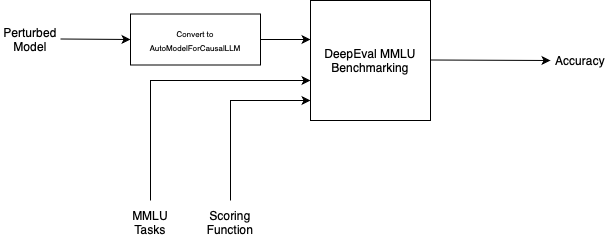
\includegraphics[width=1.0\linewidth]{images/evaluation-pipeline.png}
    \caption{Evaluation Pipeline}
    \label{fig:eval-pipeline}
\end{figure}
\subsubsection{MMLU Benchmark}
We evaluate our perturbed models on the Massive Multitask Language Understanding (MMLU) Benchmark. The MMLU Benchmark contains 15908 questions over 57 subjects. The difficulty of the questions ranges from an elementary level to an advanced professional level\cite{hendrycks2021measuringmassivemultitasklanguage}. 

For our particular evaluation framework, we narrowed the scope of our evaluation to the High School Computer Science and Astronomy tasks. The scope was narrowed from 57 tasks to 2 tasks due to the excessive computational costs required to run 15908 instances of inference on each perturbed model. These particular tasks were chosen since they provide around average performance (as seen in Figure \ref{fig:mmlu-tasks}) without exceeding the input token limit for GPT-2 and Mistral 7B.
\begin{figure}
        \centering
        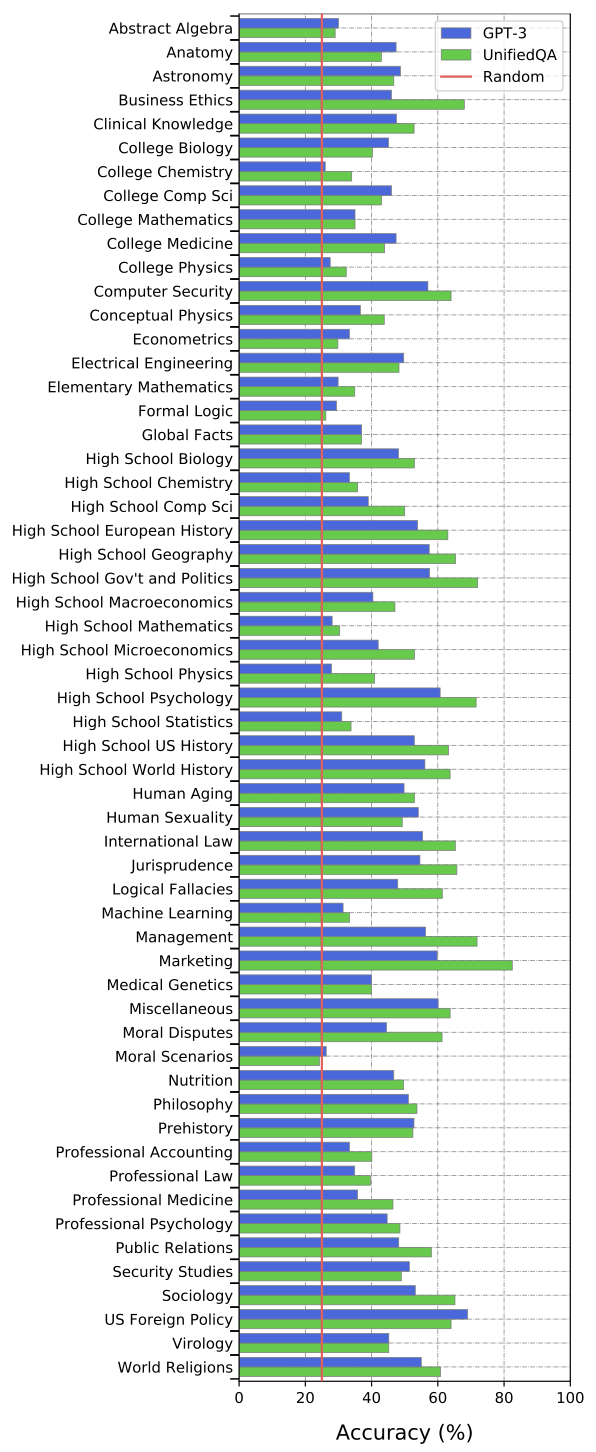
\includegraphics[width=0.75\linewidth]{images/mmlu-task-performance.png}
        \caption{Performance of GPT-3, UnifiedQA and random guessing on all 57 MMLU tasks\cite{hendrycks2021measuringmassivemultitasklanguage}}
        \label{fig:mmlu-tasks}
\end{figure}

The evaluation was conducted in a 1-shot learning setup to isolate the effect of the perturbation on the model's intrinsic knowledge retention and generalization capabilities from few-shot learning. 

\subsubsection{DeepEval Testing Framework}
In order to standardize the evaluation of the perturbed models, we used an existing library in Python called DeepEval, an open-source toolkit for LLM evaluation. The framework consists of an inbuilt class to run evaluation on particular tasks of the MMLU benchmark. 

The MMLU Benchmarking class takes as input a model, and a set of tasks to run. It then uses the following algorithm to evaluate the model on the benchmark:

\begin{algorithm}
    \caption{Evaluation algorithm for model evaluation on MMLU}
    \label{alg:eval}
    \SetAlgoLined
    \KwIn{model, tasks, score\_fn}
    \KwOut{accuracy}
    \SetKwFunction{Evaluate}{evaluate}
    \SetKwProg{Fn}{Function}{:}{}
    \Fn{\Evaluate{model, tasks, score\_fn}}{
        total\_qs $\gets$ 0\;
        total\_correct $\gets$ 0\;
        \For{task \textbf{in} tasks}{
            golden $\gets$ dataset[task]\;
            \For{g \textbf{in} golden}{
                input $\gets$ format\_input(g)\;
                result $\gets$ model.generate(input)\;
                score $\gets$ score\_fn(result, g.answer)\;
                \If{score}{
                    total\_correct $\gets$ total\_correct + 1\;
                }
                total\_qs $\gets$ total\_qs + 1\;
            }
        }
        \Return total\_correct / total\_qs\;
}
\end{algorithm}
In Algorithm: \ref{alg:eval}, the function \verb|format_input| uses a specific template to format the input to instruct the LLM to correctly answer the question in a specific format. Also, \verb|model.generate()| refers to a generic function to generate output tokens from an LLM given some set of input tokens. 

\subsubsection{Exact Match Metric}
For this evaluation framework and benchmark, we use an exact-match metric. This is a popular metric that outputs a binary result where the input is penalized if it is not an exact match to the target. In this case, we compare the output token(s) to the target, and if it is not an exact match, we return \verb|false|.

\subsection{Evaluation Framework}
\begin{enumerate}
    \item Download HuggingFace model to test on
    \item Fix an error parameter $p$ and specific labelled sections of the model to inject errors into
    \item Inject value errors with each value having probability $p$ of being an error, where our error was replacement with random value from $(0, 1)$
    \item Put our error injected model into a pipeline that conforms to the testing framework (DeepEval MMLU) in our case
    \item Run the tests and evaluate accuracy
\end{enumerate}

\subsubsection{HuggingFace Model (Mistral 7B)}
For the purpose of our experiment, we chose to use the model Mistral-7B \cite{jiang2023mistral7b} from HuggingFace and ran it using the P100 GPU provided by Kaggle.
Mistral-7B was chosen for its efficacy at relatively low memory cost. Our baseline score on our MMLU testing cases was 0.6, which is enough to be able to claim a significant difference
when injecting errors. This is compared to to GPT-2, in which even larger versions only perform at slightly better than random guessing.

A big benefit of using HuggingFace is that all layers are labelled appropriately, which makes injecting errors into specific components much easier, as we will explain later. Mistral-7B's core is made up of
32 transformer layers, each with the usual self attention, normalization, etc components.

As an aside, to be able to run on the given GPU's memory, we downloaded the model with float16 quantization. We considered further quantization but
the error injection became much more complex in this case.

\subsubsection{Error Parameters}
There are two parameters that we tried changing. An error parameter $p$ and the set of components that we wanted to inject errors into. The error parameter $p$
is the probability that a random value $p$ changes into a random value from $(0, 1)$. This process is run on every component that we want to inject errors into.

The reason we chose a random value from $(0, 1)$ is multi-fold. For one, for this specific Mistral-7B model all weights are between $(0, 1)$ so we were not losing too much
by restricting to this. The second, more important reason is that by flipping random bits, the float16 tends to explode to an extremely large value or have NaN. NaN meant that we received errors,
whereas large float16 tended to overflow and also throw an error in our code. For this reason, in order to get any results at all, we decided to stick to replacing our small weights with other small weights.

The specific error parameters that we tested were to split up all 32 layers of Mistral-7B into sublayers of size 4 (so 1-4, 5-8, etc) and inject errors into those specific sublayers. We varied $p$ logarithmically from $10^{-9}$ to $10^{-1}$.
We also looked into injecting errors into components of each layer, so we tried injecting into all self-attention layers, normalization layers, etc with the same varied values of $p$.


